\documentclass[12pt]{article} 
\usepackage[margin=1in]{geometry}
\usepackage{enumitem} %% for custom list
\usepackage{graphicx} %% for images
%\usepackage{multirow} %% for tables
%\usepackage{bigints}  %% for integrals
%\usepackage[T1]{fontenc} %% for pipe simbol
\usepackage{wrapfig} %% used to wrap img around text: https://goo.gl/SrlHQI
\usepackage{bytefield} %% for drawing packet structure
\usepackage{color} %% for color when drawing packet structure

% used for tabbed spacing
\newcommand{\itab}[1]{\hspace{0em}\rlap{#1}}
\newcommand{\tabtwo}[1]{\hspace{.2\textwidth}\rlap{#1}}
\newcommand{\tabthree}[1]{\hspace{.3\textwidth}\rlap{#1}}
\newcommand{\tabfour}[1]{\hspace{.4\textwidth}\rlap{#1}}

% using \code{come code monospaced}
\def\code#1{\texttt{#1}}

\begin{document}
\date{}
%\author{Andrea Ghizzoni \\
%some other info}
\title{\vspace{-11ex}} %% used for no title
 
\maketitle

\section{Il Livello Applicazione}\label{il-livello-applicazione}
Il livello Applicazione si colloca sulla cima del modello ISO/OSI. Tale scelta \'e dovuta alla natura del livello stesso,
ovvero di descrivere i protocolli ad alto livello che dialogano direttamente con i programmi software.

Per permettere lo scambio di messaggi tra due programmi che si trovano sulla stessa rete, \'e stata creata una semplice ma 
efficace interfaccia di programmazione al quale tutti i programmi fanno riferimento: i \textbf{socket} \textit{(dalla
terminologia Unix)}.

I socket sono un'interfaccia software messa a disposizione dal sistema operativo che permette di utilizzare in modo 
trasparente tutta l'architettura protocollare di rete. \'E analogo ad un punto di accesso/uscita SAP nel modello ISO/OSI.

Ad esempio: se un programma sulla macchina \textit{A} vorr\'a spedire un messaggio al programma destinazione sulla macchina 
\textit{B}, non dovr\'a fare altro che chiamare una utility di sistema che, in gergo, aprir\'a una socket verso la 
destinazione e rimarr\'a in attesa che A "scriva" un messaggio in essa, quindi si occuper\'a lei della consegna e gestione 
delle eventuali ritrasmissioni, riconnessioni, frammentazione dei pacchetti ecc.

Come si nota dall'esempio precedente, il software ricopre il ruolo di utilizzatore della rete, delegando ai socket tutta la 
complessit\'a del trasferimento; in altri termini presuppone l'esistenza di un'infrastruttura esterna che trasporter\'a il 
messaggio. In questo modo, nel caso di un aggiornamento del software di rete, non sar\'a necessario riscrivere ogni 
applicazione, ma baster\'a continuare a garantirle sempre la stessa interfaccia.

Una volta che il messaggio \'e arrivato a destinazione, \'e necessario un meccanismo che permetta al calcolatore di capire a 
quale processo inoltrare il messaggio. Ad ogni processo che vuole utilizzare la rete, viene quindi assegnato un numero a 16 
bit chiamato \textbf{port} dal sistema operativo.

\paragraph{Funny Story} In italiano sarebbe pi\'u corretto dire numero di \textit{porto} invece che di \textit{porta}, in
quando \'e la sua traduzione, ma nel gergo comune non \'e purtroppo utilizzato.\\\\
Esistono per\'o delle restrizioni: le porte da 0-1023 vengono chiamate \textbf{Well-known ports} \textit{(porte ben 
conosciute)} che sono definite per protocolli standard e quindi sono protette dal sistema operativo attraverso particolari 
autorizzazioni. Le porte invece da 1024-65535 sono invece lasciate per tutti gli altri applicativi che ne faranno richiesta.

\subsection{Riassumendo} Il livello applicazione permette a processi diversi di utilizzare la rete sottostante nascondendone 
tutti i dettagli implementativi; inoltre, permette di identificare ogni processo che utilizza la rete tramite un 
numero di porta.

\clearpage
\section{Architetture}\label{architetture}
Attraverso il livello applicazione, descritto in precedenza, \'e possibile categorizzare le applicazioni nel modo in cui 
comunicano tra di loro sulla rete.

\'E bene notare che si tratta solo di modelli di comunicazione, il vero protocollo \'e descritto tramite il software che lo 
implementa, che spesso \'e proprietario, e quindi non noto al pubblico. Il vantaggio di questo \'e la semplicit\'a di
sviluppo a livello applicazione di funzioni che dovrebbero essere svolte dai livelli sottostanti nella pila ISO/OSI, ad 
esempio: \'e pi\'u facile creare il proprio protocollo su HTTP in quanto non bloccato dalla maggioranza dei firewall 
presenti in internet, invece di crearlo parallelamente.

I protocolli pubblici, invece, sono descritti dagli appositi \textbf{RFC} \textit{(Request For Comments)}.

\subsection{Client-Server}\label{client-server}
Il primo modo di scambiare messaggi attraverso la rete \'e quello di inviarli ad un host centrale, il quale si occuper\'a di 
elaborarlo e di rispondere adeguatamente. In questo modello si identifica come \textbf{Client} \textit{(cliente)}, il processo 
software che invia i messaggi e \textbf{Server} \textit{(servente)} come il processo software che rimane in ascolto delle richieste 
del client per l'elaborazione.

Il server deve essere individuabile dai client in modo univoco attraverso uno o pi\'u indirizzi IP statici (che non cambiano 
nel tempo), solitamente ricavabili attraverso il sistema DNS. Il client invece non ha bisogno di un indirizzo IP pubblico, 
perch\'e il server gestir\'a l'inoltro della risposta attraverso l'indirizzo sorgente preso della richiesta. 
\begin{center}
	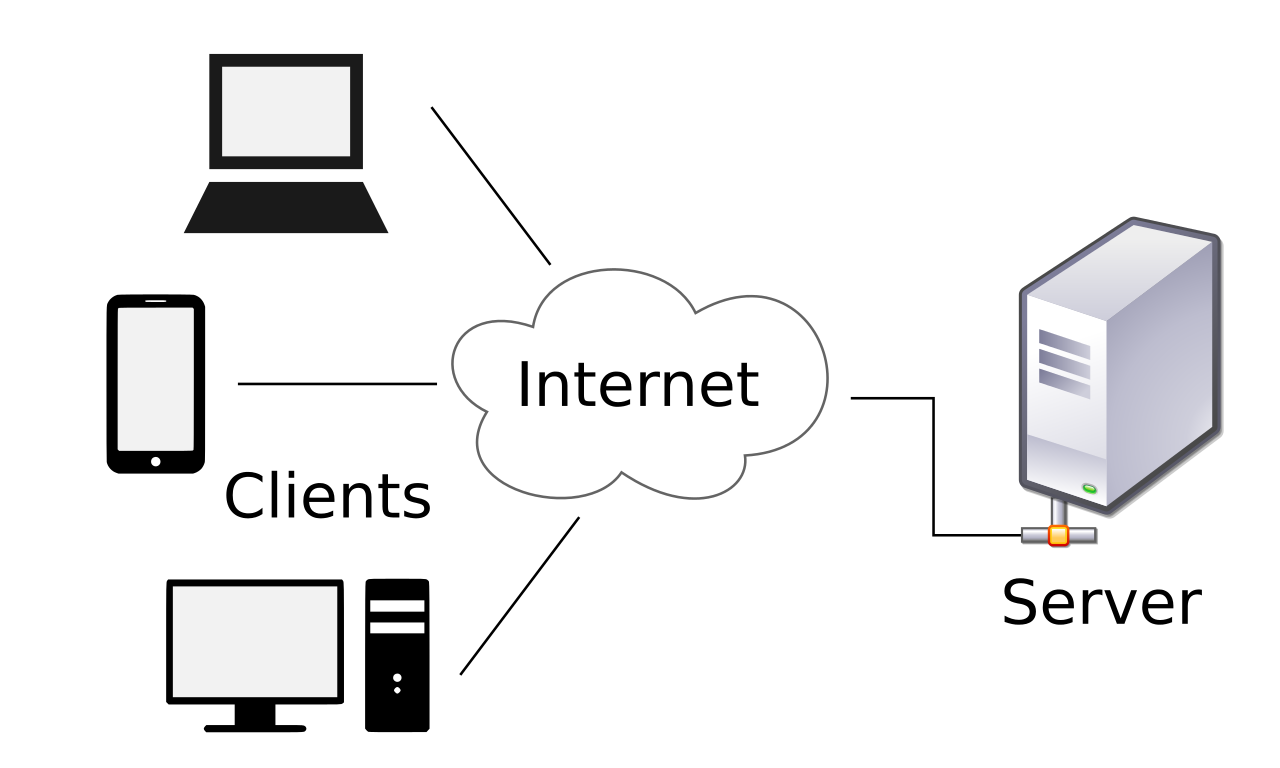
\includegraphics[scale=0.15]{applicazione-img1.png}
\end{center}
Ovviamente due client non comunicano mai tra di loro ma, ad esempio, il server potr\'a agire da tramite tra di loro.

In questo caso la complessit\'a del software risiede tutta nel server, che deve rimanere in attesa delle richieste di tutti i
client, elaborale se ben formate, ed inviare la risposta al client. Per ogni richiesta, il server deve spendere del 
tempo macchina e delle risorse per elaborare la risposta, quindi in quel momento non potr\'a accettare altre richieste. Per 
aumentare il numero di client servibili nello stesso istante l'architettura server \'e solitamente un centro di 
calcolo molto potente con il software replicato su pi\'u macchine fisiche.

Invece il client \'e un software nettamente pi\'u semplice in quanto deve solo comunicare al server che vuole iniziare una 
comunicazione, confezionare ed inviare le richieste e rimanere in attesa della risposta.

Un ulteriore modo di vedere questa architettura \'e paragonarlo al modello classico del commercio: un cliente \textit{(client)} 
che richiede un servizio al commerciante \textit{(server)}, e non il contrario.

\subsection{Peer-to-Peer o P2P}\label{p2p}
L'architettura \textbf{Peer-to-Peer}, o \textit{paritaria} o \textit{paritetica}, riprende il modello client-server ma sposta 
le resposabilit\'a del server su ogni client. Ogni host collegato nella rete, chiamato \textbf{peer} \textit{(pari)}, svolge la 
funzione sia da client che da server.

In questo modello le risorse possono essere \textbf{distribuite} su pi\'u macchine e non esiste la necessit\'a che almeno una parte 
abbia un indirizzo pubblico, in quanto nel momento della connessione tra due o pi\'u host vengono scambiati i rispettivi indirizzi 
IP.

Il vero problema riguarda la ricerca e l'indicizzazione delle risorse disponibili: un peer deve avere una visuale completa delle 
risorse presenti negli altri peer per poterli richiedere. A questo scopo si utilizzano strutture dati specifiche, come \textbf{DHT} 
\textit{(Distributed Hash Table)}.

Il vantaggio nell'utilizzo di questa architettura \'e la scalabilit\'a che si ottiene quando il numero di peer cresce condividono le 
risorse: non esiste un unico \textit{"centro" (server)} che contiene tutte le risorse, che nel caso di guasti, non sarebbero
pi\'u disponibili ai clienti, ma ogni peer pu\'o avere la sua copia della stessa risorsa e condividerla con il resto della rete.\\
\begin{center}
	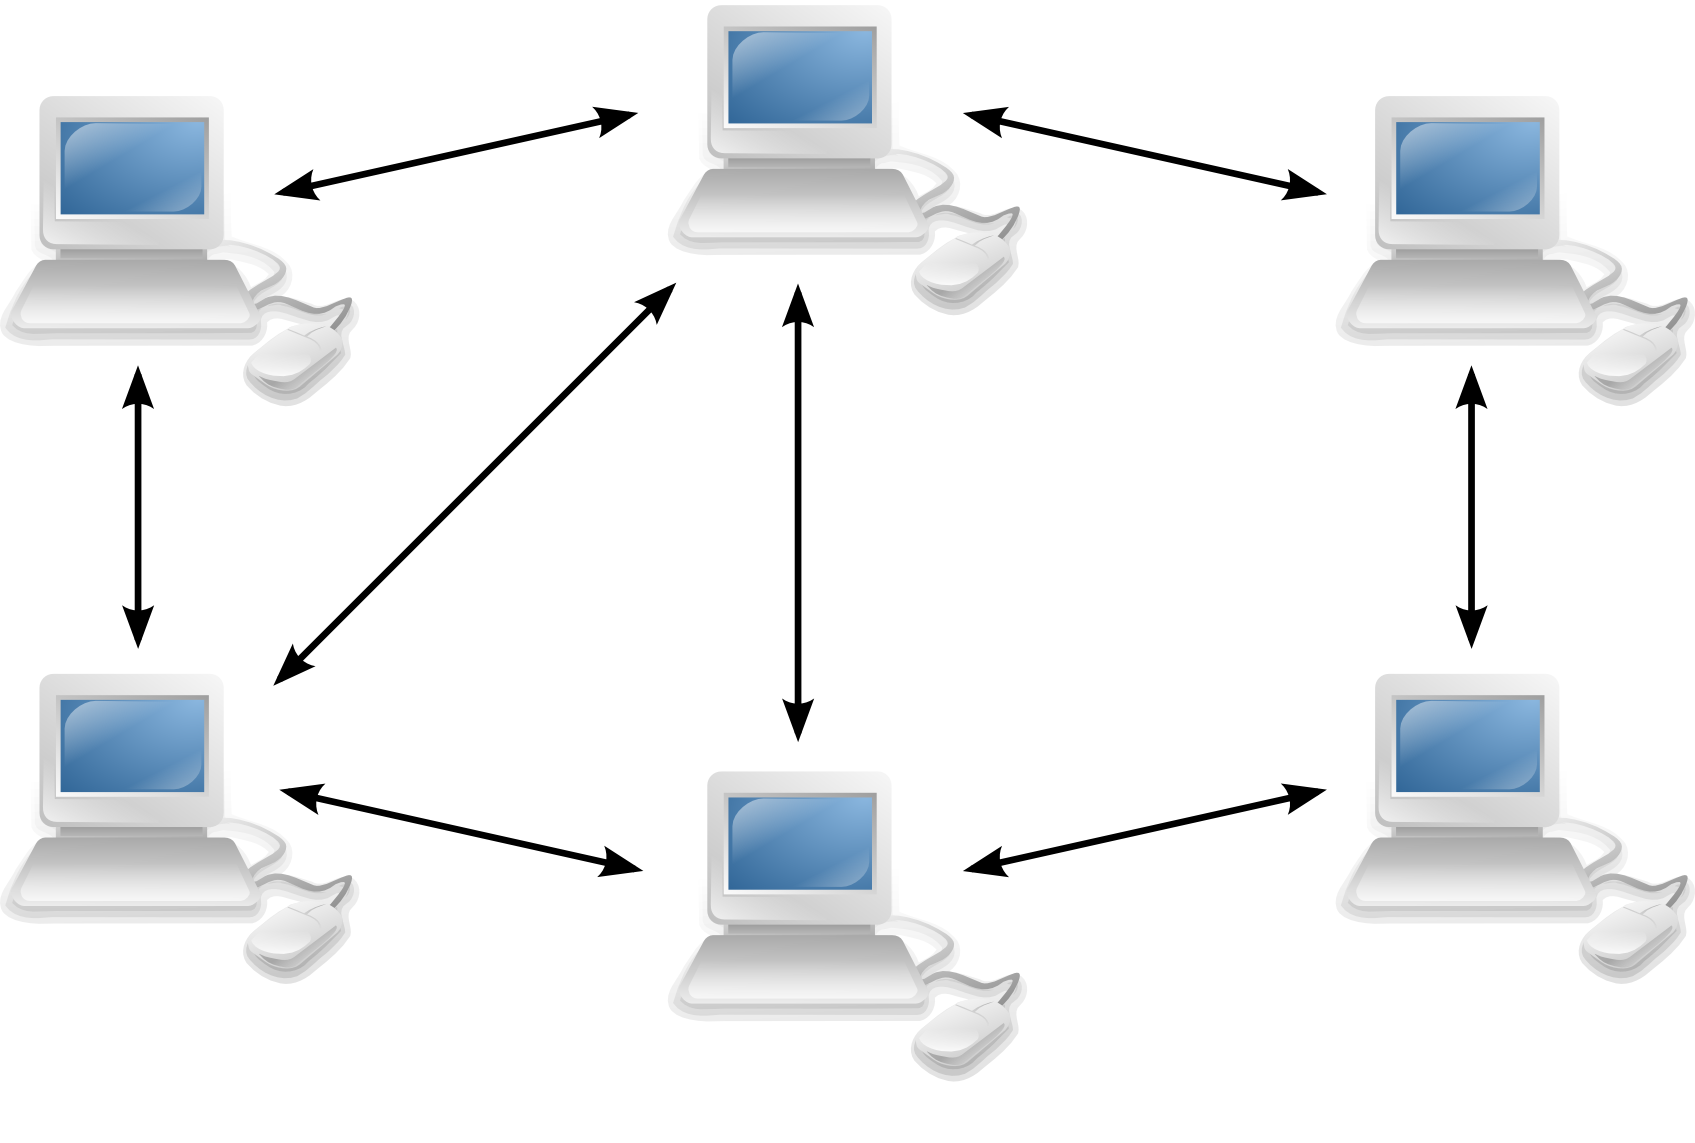
\includegraphics[scale=0.5]{applicazione-img2.png}
\end{center}

\subsection{Ibridi}\label{ibridi}
L'architettura \textbf{Ibrida} utilizza sia tecniche \textit{client-server} che \textit{peer-to-peer}, nel senso che un nuovo 
host che si collega ad una rete peer-to-peer pu\'o interrogare un server che ne contiene la locazione, in termini di indirizzi IP 
degli altri peer. In questo modo andr\'a a richiedere la risorsa direttamente all'indirizzo suggerito invece di cercarlo in tutta la 
rete.

Un esempio dell'architettura ibrida \'e stato \textbf{Skype}, un software di \textit{Voice ove IP}: principalmente usava un 
sistema client-server per l'autenticazione e un'architettura peer-to-peer per permettere la comunicazione vocale tra gli utenti.

\clearpage
\subsection{Cloud Computing}\label{cloud-computing}
L'architettura \textbf{Cloud} si pu\'o definire come l'architettura server portata all'estremo, nel senso che non esiste un 
unico host con installato il software lato server che risponde alle richieste dei client, ma esiste un'infrastruttura composta da 
molti calcolatori ad alta capacit\'a di elaborazione che viene vista come un unica macchina ad alto livello. Questo permette di 
installare il programma server con una certa quantit\'a di risorse (memoria, processori, dischi ecc) e, in caso di carico eccessivo, 
aumentarle a richiesta.

\'E possibile inoltre, se l'infrastruttura cloud lo permette, spostare l'intero software server nelle sedi vicine ai client che
richiedono i servizi. Questo \'e possibile grazie a reti specializzate della consegna di contenuti, chiamate \textbf{CDN} 
\textit{(Content Delivery Network)}. Basti a pensare a \textbf{Youtube}, ogni video che viene richiesto da un client, viene 
spostato, attraverso una CDN, nella sede Google pi\'u vicina al client per ridurre le latenze e i tempi di caricamento.
\begin{center}
	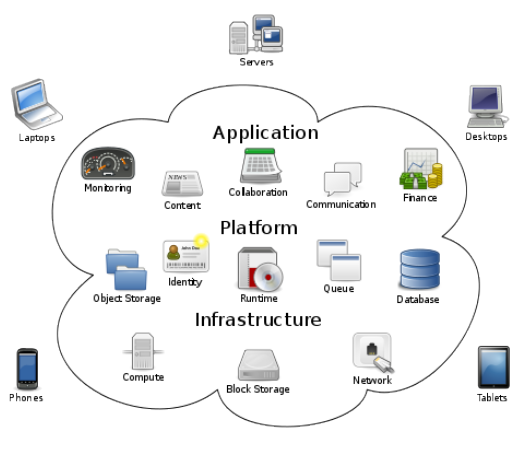
\includegraphics[scale=0.5]{applicazione-img3.png}
\end{center}
Un'ulteriore risorsa che l'infrastruttura cloud pu\'o offrire \'e la mobilit\'a d'utente: due utenti possono autenticarsi sullo 
stesso computer collegato al cloud e avere tutte le loro impostazioni e documenti disponibili, in quanto per costruzione 
dell'architettura tutte le informazioni verranno trasferite su ogni dispositivo a cui gli utenti accedono.


\clearpage
\section{DNS}\label{dns}

\subsection{La Storia}\label{dns-la-storia}
Ai tempi di ARPANET esisteva semplicemente un file, \textit{host.txt}, che manteneva tutte le associazioni tra i nomi degli host e i 
loro indirizzi IP. Ogni notte tutti i calcolatori lo prelevavano dal sito da cui era gestito. Per una rete composta da poche 
centinaia di grandi computer questo approccio era abbastanza efficace.

Tuttavia quando alla rete furono connessi milioni di PC, fu chiaro a tutti che questo metodo non poteva funzionare per sempre; 
da una parte la dimensione del file sarebbe diventata troppo elevata, mentre dall'altra cera il rischio di continui conflitti 
tra i nomi degli host.

Per risolvere questi problemi nel 1983 fu realizzato \textbf{DNS} \textit{(Domain Name System)}. L'essenza del DNS \'e 
l'introduzione di uno schema di denominazione gerarchico bastato su domini e di un database distribuito.

\subsection{Funzionamento in Breve}\label{dns-funzionamento}
Per associare un nome ad un indirizzo IP un programma applicativo invoca una procedura di libreria chiamata \textbf{resolver} 
\textit{(risolutore)}, passando il nome come parametro. Il resolver invia un pacchetto UDP contenente la richiesta a un server 
DNS locale, che cerca il nome e risponde con l'indirizzo IP \textit{(processo di risoluzione)}. Equipaggiato con l'indirizzo IP del 
destinatario cercato, il programma pu\'o quindi stabilire una connessione TCP.

\subsubsection{Lo Spazio dei Nomi}\label{dns-lo-spazio-dei-nomi}
In Internet, in cima alla gerarchia di assegnazione dei nome, c'\'e un'organizzazione chiamata \textbf{ICANN} \textit{(Internet 
Corporation for Assigned Names and Numbers)}, creato nel 1998. Concettualmente Internet \'e divisa in oltre 250 \textbf{domini 
di primo livello} o \textbf{TLD} \textit{(Top Level Domain)}. Ogni dominio \'e partizionato in \textbf{sottodomini}, che sono a loro 
volta divisi e cos\'i via.

Tutti questi domini possono essere rappresentati con una struttura ad albero, dove le foglie rappresentano i domini che non 
hanno sottodomini, ma contengono computer.
\begin{center}
	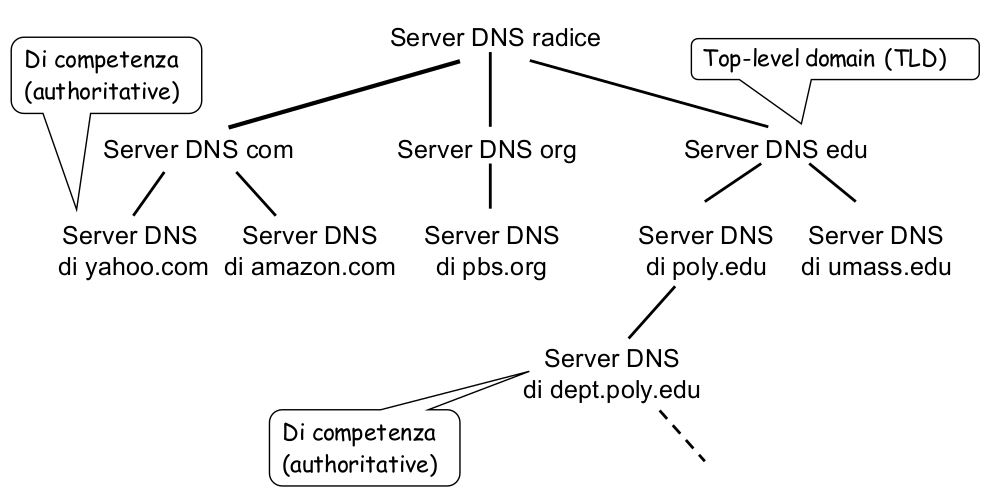
\includegraphics[scale=0.35]{applicazione-img4.png}
\end{center}
Ogni dominio \'e identificato dal percorso compreso tra esso e la radice. Le componenti sono separati da \textbf{punti} 
\textit{(dot)}. Occorre notare che questa denominazione gerarchica garantisce che, ad esempio, \textit{eng.cisco.com} non sia in 
conflitto con un potenziale utilizzo di \textit{eng} in \textit{eng.washinton.edu}, che potrebbe essere utilizzato da altri.

I componenti del nome di dominio possono essere lunghi fino a 63 caratteri, mentre il percorso completo non deve superare i 255 
caratteri.

Non esistono regole per la registrazione in due domini di primo livello della stessa societ\'a (\textit{sony.com, sony.net ..}).

La denominazione segue i confini dell'organizzazione, non le reti fisiche.

\subsubsection{Record delle Risorse di Dominio}\label{dns-record-delle-risorse-di-dominio}
A ogni dominio, che sia rappresentato da un singolo host o sia un dominio di primo livello, pu\'o essere associato un insieme di 
\textbf{resource record} \textit{(record delle risorse)} che formano il database DNS.

Quando un resolver sottopone un nome di dominio a un server DNS, ci\'o che ottiene sono i record delle risorse associate a tale 
nome. Di conseguenza la funzione principale del DNS e associare i nomi di dominio ai record delle risorse. Un record delle 
risorse \'e quindi un quintupla:
\begin{center}
	\code{Domain-name Time-to-live Class Type Value}
\end{center}

\begin{itemize}
	\item \textit{Domain-name} indica il dominio a cui si riferisce il record
	\item \textit{Time-to-live} offre un indicatore sulla stabilit\'a (o durata) del record
	\item \textit{Class} per le informazioni riguardanti Internet \'e sempre \textit{IN}
	\item \textit{Type} specifica il tipo di record tra i molti DNS
\end{itemize}
Il tipo di record pi\'u importante \'e il record \textit{A}. Contiene l'indirizzo IPv4 a 32 bit di un'interfaccia di un host. 
Alcuni host hanno due o pi\'u interfacce di rete  e in questo caso possiedono un record delle risorse di tipo A o \textit{AAAA} 
per ciascuna. Di conseguenza il DNS pu\'o fornire pi\'u indirizzi per un singolo nome.

Un altro record importante \'e il record \textit{NS} che specifica il name server per dominio o sottodominio. \'E usato come 
parte del processo di ricerca dei nomi.

I record \textit{CNAME} consentono la creazione di \textit{alias} ad esempio: se si vuole creare l'alias \textit{cs.mit.edu} per 
il dominio \textit{csail.mit.edu} il record da creare sar\'a:
\begin{center}
	\code{cs.mit.edu 86400 IN CNAME csail.mit.edu}
\end{center}
\begin{itemize}
	\item \textit{Value} che pu\'o essere un numero, un nome di dominio o una stringa ASCII.
\end{itemize}

\clearpage
\subsubsection{DNS Server}\label{dns-dns-server}
In teoria un singolo name server potrebbe contenere l'intero database DNS e rispondere a tutte le interrogazioni. In pratica, 
questo server sarebbe troppo sovraccarico per essere utile.

Per evitare problemi associati alla disponibilt\'a di un a singola fonte di informazioni, lo spazio dei nomi DNS viene diviso in 
\textbf{zone} non sovrapposte. Ogni zona \'e associata a uno o pi\'u name server. Questi sono host che tengono il database per 
la zona. Di norma, una zona avr\'a un name server primario, che contiene le sue informazioni su un file su disco e uno o pi\'u 
secondari, che ottengono le loro informazioni dal name server primario.

Il processo di ricerca di un nome e di un indirizzo \'e chiamto \textbf{risoluzione del nome}. Un \textbf{resolver} passa 
l'interrogazione a uno dei name server locali. Se il dominio \'e all'interno della giurisdizione del name server, restituisce i 
record autoritativi delle risorse. Un \textbf{record autoritativo} \'e un record fornito direttamente dall'autorit\'a che lo 
gestisce ed \'e pertanto sempre corretto.

\paragraph{Interrogazione Ricorsiva} l'interrogazione ricorsiva prevede che la risoluzione di ogni parte del nome venga gestita 
direttamente dai name server.
\begin{wrapfigure}{r}{0.45\textwidth}
  \begin{center}
    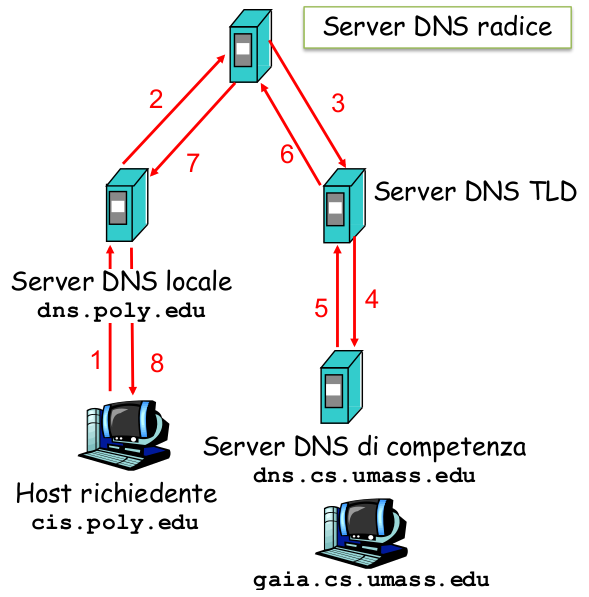
\includegraphics[scale=0.3]{applicazione-img5.png}
  \end{center}
  %\caption{app}\label{app}
\end{wrapfigure}
Come si vede dalla figura, l'host richiede la risoluzione del nome \textit{cis.poly.edu} al suo name server locale, il quale non 
conoscendolo direttamente, inoltra la richiesta di al DNS radice perch\'e viene richiesto un \textit{.edu}, il quale la inoltra 
al TLD server fino a raggiungere il name server che contiene il record desiderato. A questo punto la risposta completa torner\'a 
all'host che aveva richiesto la risoluzione.

La logica del name server locale nel supportare un'interrogazione ricorsiva \'e che sta fornendo un servizio agli host nel suo 
dominio che non devono essere configurati per svolgere essi stessi le funzioni di un name server, ma devono solo raggiungere 
quello locale. Basti a pensare ad un router casalingo che non svolge funzioni di name server, ma si appoggia sul name server 
locale.

\clearpage
\paragraph{Interrogazione Iterativa} l'interrogazione iterativa si distingue da quella ricorsiva nel nel ruolo del name server 
durante la risoluzione dell'intero nome.
\begin{wrapfigure}{r}{0.45\textwidth}
  \begin{center}
    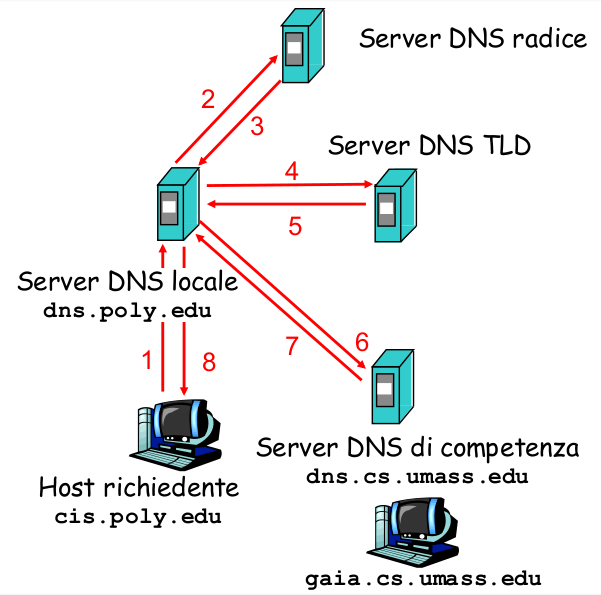
\includegraphics[scale=0.3]{applicazione-img6.png}
  \end{center}
  %\caption{app}\label{app}
\end{wrapfigure}
Come si vede nella figura, l'host richiede la risoluzione del nome \textit{cis.poly.edu} al name server locale il quale si 
preoccupa totalmente della risoluzione: chiede prima al DNS radice la risoluzione di \textit{.edu}, poi al TLD ed infine 
raggiunge il name server che contiene il dominio richiesto, che passer\'a all'host.

Il name server locale non restituisce una risposta parziale, perch\'e pur essendo utile, non \'e quello che \'e stato richiesto.

In questo caso ricoprono un ruolo molto importante i \textbf{cached record} \textit{(record archiviati nella cache)}, memorizzati 
per una certa quantit\'a di tempo per permettere la risoluzione di richieste multiple dello stesso dominio in modo pi\'u 
efficiente.

Tuttavia, le risposte archiviate nella cache non sono autoritative, perch\'e i cambiamenti fatti su un particolare dominio, non 
si propagheranno alle altre cache nel mondo. Per questa ragione le informazioni non dovrebbero vivere troppo a lungo nella cache; 
questo \'e il motivo per cui in ogni record delle risorse viene incluso un campo \textit{Time-to-live}.

Un ulteriore problema di DNS \'e il protocollo di trasporto utilizzato per le interrogazioni e le risposte: \textbf{UDP}. Non 
essendo ne connesso ne confermato, se non arriva alcuna risposta entro un limitato periodo di tempo, il client DNS ripeter\'a 
l'interrogazione, provando con un altro server del dominio dopo un piccolo numero di tentativi.


\clearpage
\section{Web e HTTP}\label{web-http}

\subsection{La Storia}\label{web-http-la-storia}
Il web nacque nel 1989 presso il CERN, il centro europeo per la ricerca nucleare. L'idea iniziale era di aiutare grandi gruppi di 
scienziati provenienti da molte nazioni anche con diversi fusi orari a collaborare utilizzando una raccolta in costante 
cambiamento di resoconti, documenti, fotografie. La proposta iniziale per una rete di documenti collegati fu opera del fisico Tim 
Berners-Lee. Il primo prototipo fu operativo 18 mesi dopo. Ne fu eseguita una presentazione pubblica nel '91 alla conferenza 
Hypertext a San Antonio, Texas. Questa dimostrazione attrasse l'attenzione di altri ricercatori a sviluppare il primo browser 
grafico, chiamato Mosaic e, successivamente Netscape.

Nel 1994 CERN e MIT firmarono un accordo per creare il \textbf{W3C} \textit{(World Wide Web Consortium)}: un'organizzazione che 
ha come scopo l'ulteriore sviluppo del Web, lo standard dei protocolli e lo sviluppo dell'interoperabilit\'a tra i siti.

Dal 1990 al 2010 i siti Web, o pagine Web sono cresciuti esponenzialmente fino a raggiungere milioni di siti e miliardi di pagine: 
\textbf{l'era del dot com}.

\subsection{Panoramica dell'architettura}\label{web-http-panoramica-architettura}
Dal punto di vista degli utenti il Web \'e una vasta raccolta mondiale di documenti o \textbf{pagine Web}, spesso definire per 
brevit\'a \textbf{pagine}. Ogni pagina pu\'o contenere collegamenti \textit{(link)} ad altre pagine situate ovunque nel 
mondo.L'idea di fare in modo che ogni pagina \textit{"puntasse"} a un'altra viene chiamato \textbf{ipertesto} \textit{(hypertext)}.

Un pezzo di testo, icona, immagine o altro, collegati ad un'altra pagina, \'e chiamato \textbf{collegamento ipertestuale} 
\textit{(hyperlink)}. Seguire il collegamento \'e un modo per indicare al browser di visualizzare un'altra pagina.

Le pagine sono visualizzate con un programma chiamato \textbf{browser} che, preleva la pagina richiesta, interpreta il testo e i 
comandi di formattazione, quindi visualizza la pagina correttamente sullo schermo. Il contenuto pu\'o essere un misto di testo, 
immagini oppure video o programmi che producono un'interfaccia grafica con cui l'utente pu\'o interagire. Ogni pagina, quindi, viene 
scaricata sulla macchina client inviando una o pi\'u richieste a uno o pi\'u server. Le domande e le risposte sono basate su un 
semplice protocollo testuale che funziona su TCP: viene chiamato \textbf{HTTP} \textit{(Hyper Text Transfer Protocol)}.

Se il documento \'e sempre uguale siamo in presenza di una \textbf{pagina statica}, mentre se \'e generato su richiesta da un 
programma o contiene del codice eseguibile \'e chiamato \textbf{pagina dinamica}.

Ogni pagina \'e descritta da un indirizzo univoco chiamato \textbf{URL} \textit{(Universal Resource Locator)} della forma:
\begin{center}
	\code{<protocollo>://<DNS/IP>/<percorso-della-risorsa>}
\end{center}
ad esempio:
\begin{center}
	\code{http://www.someschool.edu/someDept/pic.jpg}
\end{center}

\subsubsection{Il lato client}\label{web-http-il-lato-client}
In pratica, un browser \'e un programma che pu\'o visualizzare una pagina Web e rilevare i click del mouse sugli elementi in esse 
visualizzati. Quando un utente fa click su un collegamento ipertestuale il browser esegue una serie di passaggi per recuperare la 
pagina indicata:
\begin{enumerate}
	\item determina l'URL dal click dell'utente
	\item richiede al DNS l'indirizzo IP e rime in attesa della risposta
	\item il DNS risponde con l'indirizzo IP
	\item crea una connessione TCP verso l'indirizzo IP recuperato sulla porta 80
	\item invia una richiesta HTTP per la risorsa richiesta
	\item il server risponde con la risorsa richiesta
	\item se la pagina include delle URL necessarie alla visualizzazione, il browser esegue lo stesso procedimento per ognuna di 
	      queste
	\item una volta terminato l'intero scaricamento della risorsa, la visualizza
	\item la connessione TCP viene rilasciata se non vi sono altre richieste agli stessi server per un breve periodo
\end{enumerate}

\subsubsection{Il lato server}\label{web-http-il-lato-server}
Ad un server Web viene fornito il nome di un file da cercare e restituire. I passaggi eseguiti dal server nel ciclo principale 
sono i seguenti:
\begin{enumerate}
	\item accettare una connessione TCP proveniente da un client
	\item recuperare dalla richiesta HTTP il percorso della pagina
	\item ottenere il file dal disco
	\item inviare il contenuto del file al client
	\item rilasciare la connessione TCP
\end{enumerate}
Per contenuti dinamici, il terzo passaggio viene sostituito dall'esecuzione di un programma (determinato dal percorso) che 
restituisce i contenuti.

Tuttavia, i Web server possono soddisfare molte richieste al secondo. Il problema \'e che l'accesso al disco \'e spesso il collo 
di bottiglia: gli stessi file possono essere letti ripetutamente dal disco usando chiamate al sistema operativo. Ulteriormente, nel momento in cui il server legge un file dal disco, potenzialmente di grandi dimensioni, non pu\'o accettare nessun'altra connessione.

Un miglioramento ovvio consiste nel mantenere in cache gli \textit{n} file utilizzati pi\'u di recente o un certo 
numero di gigabyte di contenuti. Prima di accedere al disco per recuperare il file, il server controlla la cache. Se il file \'e 
presente, pu\'o essere inviato direttamente dalla memoria. 

Per ovviare al problema di servire una singola richiesta alla volta, una strategia \'e implementare il server con un approccio 
\textbf{multithread}: un thread, detto di \textbf{front-end} rimane in ascolto delle richieste dei client ed esegue operazioni di 
\textbf{load-balancing}, ovvero ridirige la richiesta su un'altra macchina, la quale gestir\'a in pieno la richiesta.
\begin{center}
    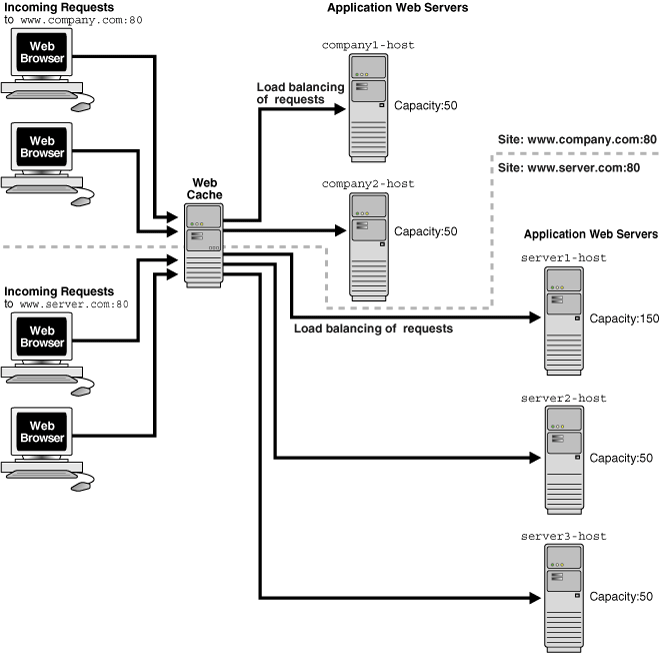
\includegraphics[scale=0.55]{applicazione-img7.png}
\end{center}
Ovviamente questo schema \'e di pi\'u complessa realizzazione, ma necessario quando cresce il numero di utenti.
La macchina incaricata deve quindi:
\begin{enumerate}
	\item risolve il nome della pagina Web richiesta
	\item eseguire il controllo di accesso alla pagina
	\item controllare la cache
	\item prelevare la pagina richiesta dal disco o eseguire un programma che la costruisca
	\item determinare il resto della risposta
	\item restituire la risposta al client
	\item aggiungere un elemento al registro delle operazioni svolte dal server
\end{enumerate}

\subsection{HTTP}\label{web-http-http}
Il protocollo usato per trasportare informazioni tra server Web e client \'e \textbf{HTTP} \textit{(Hyper Text Transfer 
Protocol)}. HTTP \'e un protocollo basato sul modello di domanda e risposta \textit{(request-response)}, normalmente implementato 
su TCP. Specifica quali messaggi i client possono inviare ai server e quali risposte vengono restituite. Le intestazioni delle 
domande e delle risposte sono formulate in ASCII.

HTTP sta diventando sempre pi\'u un protocollo di trasporto, ovvero che rende possibile ai processi lo scambio di contenuti 
attraverso reti differenti. Questi processi potrebbero anche non essere un browser Web o un server Web; ad esempio gli 
sviluppatori possono impiegare HTTP per il recupero di file di progetto.

\subsubsection{Connessioni}\label{web-http-http-connessioni}
Il modo solitamente utilizzato dal browser per contattare un server prevede di stabilire una connessione TCP sulla porta 80 al 
suo indirizzo. Il vantaggio di TCP sta nel fatto che n\'e i browser ne i server devono preoccuparsi dei messaggi lunghi, 
affidabilit\'a o controllo di congestione, in quanto sono gestiti dall'implementazione di TCP.

Con HTTP 1.0 le pagine erano generalmente composte da un unico file html quindi, dopo aver stabilito la connessione, veniva inviata 
una singola richiesta e restituita una singola risposta; a questo punto la connessione TCP veniva rilasciata. Nel giro di pochi 
anni la pagina Web media inizi\'o a contenere sempre pi\'u collegamenti a contenuti, quali icone e altri elementi per migliorarne 
l'aspetto, ma stabilire una connessione TCP per trasportare una singola icona diventava un modo molto costoso di operare.

Questa osservazione ha portato ad HTTP 1.1, che supporta \textbf{connessioni persistenti}. Con questa tecnologia \'e possibile 
stabilire una connessione TCP, inviare una richiesta, ottenere una risposta e poi inviare altre richieste e ottenere nuove 
risposte. Questa strategia \'e detta \textbf{riutilizzo della connessione}.\footnote{RTT \textit{(Round Trip Time)}: tempo impiegato dall'unit\'a dati per arrivare alla destinazione e ritorno}
\begin{center}
    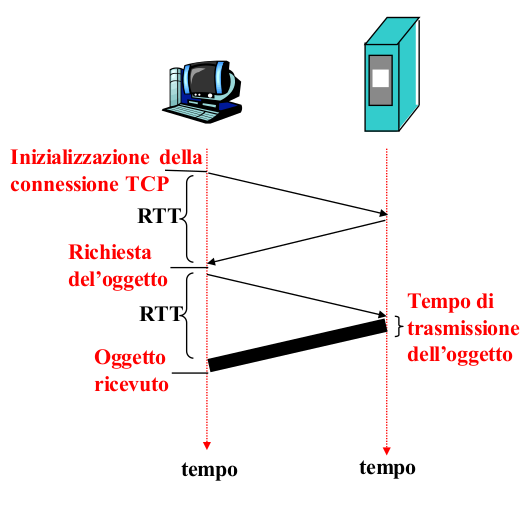
\includegraphics[scale=0.4]{applicazione-img8.png}
\end{center}

\subsubsection{Messaggi e Metodi}\label{web-http-http-messaggi-e-metodi}
Anche se HTTP fu progettato per l'utilizzo sul Web \'e stato reso intenzionalmente pi\'u generico del necessario per permettere 
alle applicazioni future di svilupparsi. Per questo motivo sono supportate varie operazioni chiamate \textbf{metodi}.

Ogni richiesta consiste di una o pi\'u righe di testo ASCII, con la prima parola della prima riga che rappresenta il nome del 
metodo richiesto. Esistono diversi metodi, i pi\'u comuni sono:
\begin{itemize}
	\item \code{GET} richiede al server l'invio di un file attraverso, anche dei parametri specificati nell'URL dopo il carattere
	di escape \code{?}. Ad esempio:\\
	%\begin{center}
		\centerline{\code{http://www.someurl.edu/res.txt?a=1\&b=2}}\\
	%\end{center}
	richiede al server il file \code{res.txt} con i parametri \code{a=1} e \code{b=2}.
	
	\item \code{POST} stessa funzione di \code{GET} con la differenza che accoda dei possibili parametri ai dati del messaggio 
	invece che nella URL.

	\item \code{PUT} \'e il contrario di \code{GET}: invece di leggere la pagina, la scrive.

	\item \code{HEAD} richiede solamente l'intestazione del messaggio, senza la pagina effettiva. Questo metodo pu\'o essere 
	utilizzato per ottenere la data dell'ultima modifica di una pagina, per raccogliere informazioni a scopo di indicizzare o per 
	verificare la validit\'a di un URL.

	\item \code{DELETE} rimuove la pagina o almeno indica che il server web \'e d'accordo a rimuovere la pagina. Autenticazione e 
	autorizzazione giocano un ruolo fondamentale.\\ %% this new line is for better layout
\end{itemize}

Ogni richiesta ottiene una risposta costituita da una riga di stato e magari da altre informazioni. La riga di stato contiene un 
codice di tre cifre che indica se la richiesta \'e stata soddisfatta e, in caso contrario, la causa del fallimento.

Le famiglie di codici si dividono in:
\begin{itemize}[noitemsep]
	\item \code{1xx} Informazione
	
	\item \code{2xx} Successo
		  \begin{itemize}[noitemsep]
		      \item \itab{\code{200 OK}}         \tabfour{richiesta andata a buon fine}
		  	  \item \itab{\code{204 No Content}} \tabfour{nessun contenuto trovato}
		  \end{itemize}
		  
	\item \code{3xx} Redirezione
		  \begin{itemize}[noitemsep]
		  	   \item \itab{\code{301 Moved Permanently}} \tabfour{pagina spostata}
		  \end{itemize}
	
	\item \code{4xx} Errore del Client
		  \begin{itemize}[noitemsep]
		  	   \item \itab{\code{400 Bad Request}} \tabfour{richiesta malformata}
		  	   \item \itab{\code{404 Not Found}}   \tabfour{contenuto non trovato}
		  \end{itemize}
		  
	\item \code{5xx} Errore del Server
	      \begin{itemize}[noitemsep]
		  	   \item \itab{\code{500 Internal Server Error}} \tabfour{errore interno al server}
		  	   \item \itab{\code{503 Service Unavailable}}   \tabfour{servizio non disponibile}
		  \end{itemize}
\end{itemize}

Di seguito un esempio di richiesta HTTP:\\\\
% using \itab and  \tabthree to keep text alligned in the center of the page
\itab{} \tabthree{\code{GET /somedir/page.html HTTP/1.1}}\\
\itab{} \tabthree{\code{Host: www.someschool.edu}}\\
\itab{} \tabthree{\code{User-agent: Mozilla/4.0}}\\
\itab{} \tabthree{\code{Connection: close}}\\
\itab{} \tabthree{\code{Accept-language: it}}\\

Di seguito un esempio di risposta HTTP:\\\\
% using \itab and  \tabthree to keep text alligned in the center of the page
\itab{} \tabthree{\code{HTTP/1.1 200 OK}}\\
\itab{} \tabthree{\code{Connection: close}}\\
\itab{} \tabthree{\code{Date: Thu, 06 Aug 1998 12:00:15 GMT}}\\
\itab{} \tabthree{\code{Server: Apache/1.3.0 (Unix)}}\\
\itab{} \tabthree{\code{Last-Modified: Mon, 22 Jun 1998}}\\
\itab{} \tabthree{\code{Content-Length: 6821}}\\
\itab{} \tabthree{\code{Content-Type: text/html}}\\
\itab{} \tabthree{\code{\dots dati utente \dots}}\\\\ % duble newline for better impagination

Si pu\'o generalizzare la richiesta o risposta HTTP come segue:\\
\begin{center}
	\begin{bytefield}{32}
		\begin{rightwordgroup}{header}
			\begin{leftwordgroup}{richiesta}
				\bitbox{8}{metodo}    & \bitbox{2}{sp} & 
				\bitbox{8}{URL}       & \bitbox{2}{sp} & 
				\bitbox{8}{versione}  & \bitbox{2}{cr} & \bitbox{2}{lf}
			\end{leftwordgroup}\\
			\begin{leftwordgroup}{risposta}
				\bitbox{8}{versione} & \bitbox{2}{sp} &
				\bitbox{18}{codice}  & \bitbox{2}{cr} & \bitbox{2}{lf}
			\end{leftwordgroup}\\
			\bitbox{17}{nome campo header} & \bitbox{1}{:} & \bitbox{10}{valore} & \bitbox{2}{cr} & \bitbox{2}{lf} \\
			\wordbox[]{1}{$\vdots$} \\[1ex]
			\bitbox{17}{nome campo header} & \bitbox{1}{:} & \bitbox{10}{valore} & \bitbox{2}{cr} & \bitbox{2}{lf} 		
		\end{rightwordgroup}\\
		\bitbox{2}{cr} & \bitbox{2}{lf} \\
		\begin{rightwordgroup}{corpo del\\messaggio}
			\wordbox{3}{dati}
		\end{rightwordgroup}
	\end{bytefield}
\end{center}

\paragraph{Da Notare:} Ogni parte del messaggio viene separata dai caratteri \textbf{carriage return (cr)} \textit{(cursore ad 
inizio riga)} e \textbf{line field (lf)} \textit{(cursore spostato nella riga sottostante)}.
Per separare le parti della prima riga si utilizza un \textbf{separatore (sp)}, solitamente uno spazio.

\clearpage% for pagination
\subsubsection{I Cookie}\label{web-http-http-i-cookie}
Navigare per il Web comporta il recupero di una serie di pagine indipendenti: il browser invia una richiesta a un server, ottiene il 
file, dopo di che il server dimentica di aver mai visto quel particolare client. Questo comportamento viene chiamato comportamento 
\textbf{stateless} \textit{(senza stato)}.

Tuttavia esso non \'e adatto per fornire pagine differenti a utenti diversi a seconda dell'interazione avuta in precedenza col 
server. Questo comportamento \'e necessario per molti sistemi che prevedano una sequenza logia di scambi di informazioni con i 
siti Web, per esempio: alcuni siti Web richiedono agli utenti di registrarsi oppure per rendere l'esperienza sul sito pi\'u 
gradevole.

Questo fa nascere il problema di come possono i server distinguere tra le richieste dei vari utenti. Il problema fu risolto col 
meccanismo, spesso criticato, dei \textbf{cookie} \textit{(biscotti)}, inventati da Netscape nel 1994.

Quando un client richiede una pagina Web il server pu\'o fornire informazioni aggiuntive sotto forma di cookie insieme alla pagina 
richiesta. Un cookie \'e un piccolo file (circa 4KB) che il server pu\'o associare a un browser. I browser archiviano i cookie in 
un'apposita directory sul disco rigido del client, a meno che l'utente non li abbia disattivati. I cookie potrebbero teoricamente 
contenere un virus, ma visto che sono trattati come dati testuali, non esiste un modo ufficiale per mandare in esecuzione 
l'ipotetico virus.

Un cookie \'e composto dai seguenti campi:
\begin{center}
	\code{Dominio-Percorso-Contenuto-Scadenza-Sicuro}
\end{center}
dove:
\begin{itemize}[noitemsep]
	\item \code{Dominio} indica il nome del dominio da dove proviene
	\item \code{Percorso} \'e un percorso nella struttura delle directory del server che identifica quale parte della struttura di 
		  file del server pu\'o utilizzare il cookie
	\item \code{Contenuto} campo sotto forma di \textit{chiave = valore}
	\item \code{Scadenza} specifica quando scade il cookie. Se il campo \'e assente, il browser scarta il cookie alla sua 
		  chiusura: un cookie di questo tipo \'e definito \textbf{cookie non persistente}. Se vengono fornite una data e un'ora, il 
		  cookie \'e \textbf{persistente} ed \'e conservato fino alla scadenza.
	\item \code{Sicuro} pu\'o essere impostato per indicare che il browser pu\'o restituire il cookie a un server solo usando un 
	      sistema di trasporto sicuro.
\end{itemize}
Il browser, prima di inviare una richiesta di una pagina Web, cerca nell'apposita directory tutti i cookie inseriti con dominio 
uguale al dominio richiesto. Se la ricerca porta dei risultati, vengono inclusi nel messaggio di richiesta. Quando il server li 
riceve, pu\'o interpretarli come desidera.

Un impiego pi\'u controverso \'e quello di tracciare il comportamento on-line degli utenti. Questo permette agli 
operatori di siti Web di capire come gli utenti navigano nel loro sito; le aziende pubblicitarie costruiscono profili di 
pubblicit\'a o siti che un particolare utente ha visitato. Purtroppo molti utenti sono completamente inconsapevoli di questa 
collezione di informazioni, a volte anche riguardante l'indirizzo mac o il browser utilizzato, oppure la lingua e il sistema 
operativo.

\subsubsection{Proxy Web}\label{web-http-http-proxy-web}
Una strategia per aumentare l'efficacia delle cache consiste nel condividerle tra pi\'u utenti. In questo modo una pagina gi\'a  
richiesta da un utente pu\'o essere restituita ad un altro senza che la richiesta raggiunga effettivamente il web server. 
Naturalmente questa condivisione non pu\'o essere fatta per: traffico codificato, pagine che richiedono l'autenticazione e per 
pagine che sono restituite da programmi.

Un \textbf{Proxy Web} \'e usato per fare condivisione di cache tra utenti. Un proxy, generalmente, \'e un agente che agisce in vece 
di qualcuno, per esempio l'utente, occupandosi delle richieste Web al posto dei suoi utenti.

\begin{center}
    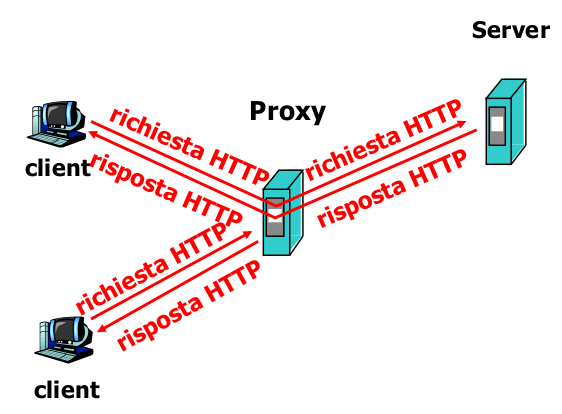
\includegraphics[scale=0.5]{applicazione-img9.png}
\end{center}

Per usare il proxy ogni browser deve essere configurato in modo da fare le richieste delle pagine al proxy invece che al vero 
server. Se il proxy ha la pagina, la gestisce immediatamente; altrimenti, prende la pagina dal server, la memorizza nella cache per 
usarla ancora in futuro e la restituisce al client che l'ha richiesta. Il proxy viene consultato solo dopo che il browser abbia 
tentato di soddisfare la richiesta usano la propria cache.\\
Quindi il proxy determina:
\begin{itemize}[noitemsep]
	\item un miglioramento del tempo di risposta delle risorse Web
	\item riduce il traffico verso internet, cruciale quando la tariffazione della linea \'e svolta tramite conteggio della banda 
	      utilizzata dagli utenti.
	\item pu\'o filtrare i contenuti 
	\item garantisce l'anonimato dell'utente dal server
\end{itemize}

\paragraph{Proxy $\neq$ NAT} La differenza tra Web proxy e NAT \'e che il primo possiede la nozione semantica dell'applicazione, 
ovvero esiste un proxy che esegue le richieste per ogni tipo di applicazione, invece il NAT avviene a livello di rete, ovvero per 
ogni comunicazione che avviene nei livelli superiori, viene eseguito la traduzione di indirizzo.


\clearpage
\section{Posta Elettronica}\label{posta-elettronica}
La \textbf{Posta Elettronica} \textit{(e-mail)} \'e disponibile da pi\'u di tre decenni. Pi\'u veloce ed economica della posta 
tradizionale, l'e-mail \'e stata un'applicazione popolare fin dai primi esordi di Internet. Prima del 1990 era utilizzata 
principalmente nella universit\'a. Successivamente \'e divenuta nota al grande pubblico ed \'e cresciuta in modo esponenziale. 
Sfortunatamente, come per le lettere cartacee, la maggior parte delle e-mail, 9 su 10, \'e costituita da \textbf{spam} 
\textit{(messaggi spazzatura)}.

I protocolli e-mail si sono evoluti nel corso  degli anni. I primi sistemi di posta elettronica erano semplicemente protocolli di 
trasferimento per file testuali, con la convenzione che la prima riga di ogni messaggio (o file) conteneva l'indirizzo del 
destinatario. Con il trascorrere del tempo l'e-mail si \'e diversificata dal trasferimento file e sono state aggiunte molte 
propriet\'a, quali la capacit\'a di inviare un messaggio a una lista di destinatari. Negli anni '90 divennero importati le 
funzionalit\'a multimediali per inviare messaggi contenenti immagini o altro materiale non testuale. Anche i programmi di lettura 
delle e-mail divennero pi\'u sofisticati, spostandosi da interfacce basate sul testo a interfacce grafiche e aggiungendo la 
possibilit\'a di accedere alla proprie e-mail da qualsiasi computer ovunque ci si trovi.

\subsection{Architettura e Servizi}\label{posta-elettronica-architettura-e-servizi}
\begin{center}
    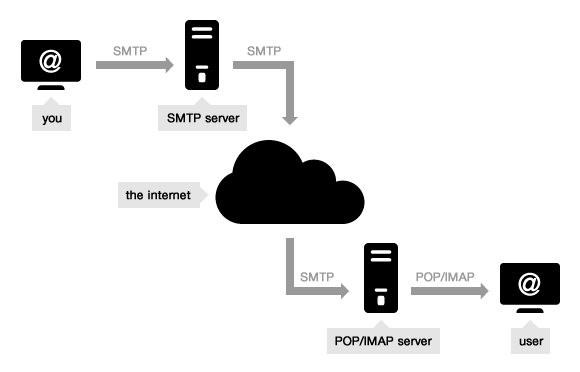
\includegraphics[scale=0.5]{applicazione-img10.png}
\end{center}
L'architettura del sistema \'e composta da due sottosistemi: gli \textbf{user agent}, che consentono alle persone di leggere e 
inviare la posta elettronica, e i \textbf{message transfer agent}, che spostano i messaggi dalla sorgente alla destinazione. Questi 
ultimi sono informalmente chiamati \textbf{mail server}.

Alcune elaborazioni dello user agent possono essere fatte automaticamente: le e-mail in ingresso possono essere filtrate o attribuire 
una minore priorit\'a ai messaggi che potrebbero essere spam.

I message transfer agent sono tipicamente processi di sistema. Vengono eseguiti come servizi su appositi server e sono pensati per 
essere sempre disponibili. Il loro compito \'e di spostare automaticamente  le e-mail attraverso il sistema della sorgente al 
destinatario facendo uso del protocollo SMTP.

SMTP invia le e-mail con un approccio orientato alla connessione e notifica lo stato della consegna e degli errori.

I message transfer agent implementano anche le \textbf{mailing list}, in cui copie identiche di un messaggio vengono consegnate a ogni 
iscritto alla lista. Altre funzionalit\'a avanzate sono le copie per conoscenza \textit{(carbon copy, cc)}, le copie per conoscenza 
nascosta \textit{(blind carbon copy, bcc)}, i messaggi di posta elettronica ad alta priorit\'a.

I concetti di \textbf{mailbox} \textit{(caselle di posta)} e di formato standard dei messaggi e-mail sono il collegamento tra user 
agent e message transfer agent. Le mailbox memorizzano le e-mail ricevute dall'utente e sono mantenute dai mail server, mentre gli 
user agent semplicemente presentano agli utenti una visione  dei contenuti delle loro mailbox. Per fare ci\'o, gli user agent inviano 
ai mail server i comandi per manipolare le mailbox, ispezionando i loro contenuti, cancellando messaggi e cos\'i via. Con questa 
architettura per accedere a una mailbox un utente pu\'o usare differenti user agent su diversi computer.

Un'idea basilare nei sistemi di posta elettronica \'e la distinzione tra l'\textit{involucro} e il suo contenuto. L'involucro 
incapsula il messaggio e contiene tutte le informazioni necessarie per il suo trasporto, come l'indirizzo di destinazione, la 
priorit\'a e il livello di protezione. I message transfer agent utilizzano l'involucro per l'instradamento.

Il messaggio all'interno dell'involucro consiste in due parti: l'\textit{intestazione} e il \textbf{corpo}. L'intestazione contiene 
informazioni di controllo per gli user agent, mentre il corpo \'e dedicato interamente al destinatario umano.

\subsection{User Agent}\label{posta-elettronica-user-agent}
Uno user agent \textit{(o e-mail reader o client di posta)} \'e un programma che accetta una variet\'a di comandi per comporre, 
ricevere e rispondere ai messaggi, nonch\'e per organizzare le caselle di posta. Ci sono molti user agent popolari quali Google 
Gmail, Microsoft Outlook e Mozzilla Thunderbird.

Gli user agent devono anche essere in grado di mostrare i messaggi in arrivo in modo che le persone possano leggere le proprie e-mail 
e, successivamente, decidere cosa farne: distruggerlo, inviare una risposta, inoltrare il messaggio o conservarlo.

L'archiviazione pu\'o essere fatta automaticamente dallo stesso user agent prima che l'utente legga i messaggi. Un esempio comune si 
ha quando i campi e i contenuti dei messaggi sono ispezionati e usati, insieme a quanto detto dall'utente riguardo ai messaggi 
precedenti, per determinare se un messaggio pu\'o essere spam. Molti ISP e aziende fanno uso di software che etichetta le e-mail come 
importanti o spam in modo che lo user agent possa archiviarle nella casella di posta corrispondente.

Gli utenti possono costruirsi delle regole di archiviazione. Ogni regola specifica una condizione e un'azione. Le cartelle pi\'u 
importanti sono la \textit{Inbox} e la \textit{Junk e-mail}.

Una propriet\'a di base degli user agent \'e come comporre le e-mail. Questa include la creazione di messaggi o risposte a messaggi e 
l'invio del tutto nel sistema di e-mail per la consegna. I messaggi inviati hanno un formato standard che viene creato a partire 
dalle informazioni fornite dallo user agent. La parte pi\'i importante del messaggio per il trasferimento \'e l'involucro, che 
contiene l'indirizzo della destinazione nella forma \textit{user@indirizzo-dns}.

\subsection{Trasferimento dei Messaggi}\label{posta-elettronica-trasferimento-dei-messaggi}
Il trasferimento delle e-mail \'e fatto dal protocollo \textbf{SMTP} \textit{(Simple Mail Transfer Protocol)}. Il modo pi\'u semplice 
per svolgere questa operazione \'e stabilire una connessione di trasporto della macchina sorgente a quella destinazione per poi 
trasferire semplicemente il messaggio. Cos\'i faceva originariamente SMTP. Tuttavia nel corso degli anni, si sono differenziati due 
diversi tipi di uso di SMTP. Il primo \'e la sottomissione della mail, modo in cui lo user agent invia messaggi nel sistema e-mail 
per la consegna, il secondo consiste nel trasferire direttamente i messaggi ai message transfer agent del destinatario.

\subsubsection{SMPT e le sue estensioni}\label{posta-elettronica-smtp-ed-estensioni}
All'interno di Internet la posta elettronica viene consegnata costituendo una connessione tra la macchina sorgente e la porta 25 
della macchina di destinazione. In ascolto su questa porta esiste un server di posta elettronica che utilizza \textbf{SMTP}.

SMTP \'e un semplice protocollo ASCII. Usare testo ASCII facilita lo sviluppo dei protocollo e il relativo debug: possono essere 
validati inviando comandi composta manualmente de i record dei messaggi sono facili da leggere. La maggior parte dei protocolli 
Internet di livello applicazione funzionano in questo modo.

SMTP nella sua forma base funziona bene, ma \'e limitato in alcuni aspetti: non include l'autenticazione, trasferisce i messaggi in 
ASCII e, soprattutto, in chiaro. Per risolvere questi problemi SMPT \'e stato rivisto per avere un meccanismo di estensioni. L'uso di 
SMTP con tali estensioni \'e chiamato \textbf{ESMTP} \textit{(Extended SMTP)}.

\subsubsection{Sottomissione delle e-mail}\label{posta-elettronica-sottomissione-delle-email}
SMTP \'e normalmente usato per la sottomissione della e-mail con l'estensione \textit{AUTH}, che permette al server di controllare le 
credenziali di accesso al servizio di posta elettronica del client.

Ci sono ulteriori differenze nel modo in cui SMTP \'e usato per la sottomissione della posta. Per esempio, la porta 587 \'e preferita 
alla porta 25 e il server SMTP pu\'o controllare e correggere il formato dei messaggi inviati dallo user agent.

\subsubsection{Message Transfer}\label{posta-elettronica-message-transfer}
Quando un message transfer agent riceve un messaggio da uno user agent, lo consegner\'a al message transfer agent del destinatario 
usando SMTP. Per fare ci\'o la sorgente usa l'indirizzo di destinazione.

Per determinare il corretto server di posta elettronica da contattare viene interrogato il sistema DNS riguardante il record MX 
\textbf{(o mail exchanger)} del dominio, restituendo una lista ordinata degli indirizzi IP di uno o pi\'u server di posta 
elettronica. Il message transfer agent sorgente stabilisce quindi una connessione TCP sulla porta 25 verso l'indirizzo IP cos\'i 
ottenuto e usa SMTP per consegnare il messaggio. Il ricevente quindi metter\'a l'e-mail nella corretta casella di posta dell'utente.

Con questo processo di consegna la posta viaggia dal message transfer agent iniziale a quello finale con un solo salto. Non ci sono 
server intermedi nel trasferimento di messaggi.

\subsection{Consegna Finale}\label{posta-elettronica-consegna-finale}
La e-mail una volta arrivata alla casella di posta non rimane altro che trasferirne una copia allo user agent dell'utente per essere 
visualizzata. I compiti dello user agent sono quelli di visualizzare i contenuti della casella di posta e permettere che venga 
gestita da remoto. A questo scopo possono essere usati diversi protocolli differenti, ma non SMTP, che \'e un protocollo di 
\textit{push}\footnote{Un protocollo che quindi "spinge" \textit{(push)} i dati verso la destinazione in contrapposizione ai 
protocolli di \textit{pull} che invece li attirano a s\'e.}.

La consegna finale non pu\'o essere eseguita in questo modo, sia perch\'e la casella di posta deve continuare ad essere memorizzata 
sul mail server sia perch\'e lo user agent potrebbe non essere connesso ad Internet nel momento in cui SMTP tenta di inoltrare i 
messaggi.

\subsubsection{IMAP e POP3}\label{posta-elettronica-imap-pop3}
Uno dei protocolli principali usati per la consegna finale \'e \textbf{IMAP} \textit{(Internet Message Access Protocol)}. Per fare 
uso di IMAP il mail server esegue un server IMAP che rimane in ascolto sulla porta 143. Lo user agent esegue la versione client di IMAP che si connette al server e inizia la comunicazione.

Innanzitutto il client instaura una sessione di trasporto sicura e quindi effettua il login o un'altra autenticazione sul server. Una 
volta autenticato esistono molto comandi per elencare le cartelle e i messaggi, per prendere i messaggi o parte di essi, etichettarli 
per una successiva cancellazione e organizzarli in cartelle.

IMAP \'e un aggiornamento di un protocollo di consegna finale precedente, \textbf{POP3} \textit{(Post Office Protocol version 3)}. 
Invece di rimanere sul server i messaggi sono solitamente scaricati dallo user agent del computer. Questo facilita la vita ai server, 
ma la complica agli utenti.

Tuttavia POP3 viene ancora usato. Possono essere usati anche protocolli proprietari, perch\'e il protocollo pu\'o essere impiegato 
tra server di posta elettronica e user agent forniti dalla stessa azienda; Microsoft Exchange \'e un sistema di e-mail con protocollo 
proprietario




\end{document}